\chapter[Desenvolvimento]{Desenvolvimento}

	Este capítulo descreve os passos para a realização deste trabalho, mostrando desde os equipamentos utilizados até os procedimentos de implementação, coleta e análise dos dados. 

\section{Levantamento Bibliográfico}

Uma vez escolhida a área de interesse e o tema, a primeira etapa do trabalho consistiu em um levantamento bibliográfico, a fim de avaliar a disponibilidade de material para fomentar o tema do trabalho e também analisar o que já foi publicado e desenvolvido na área. Feito isto, foram definidas as possíveis contribuições, identificando (como foi dito no Capítulo \ref{introduc}) a limitação de desempenho e o desenvolvimento para \textit{mobile} como áreas a serem exploradas.  

\section{Equipamentos Utilizados}
\label{equip}

	 O computador utilizado para o desenvolvimento na plataforma \textit{Android} foi o da linha \textit{Alienware} M14x fabricado pela \textit{Dell}, no qual possui processador \textit{Intel Core} i7 de 2,3 GHz, GPU \textit{NVIDIA GeForce} GTX de 2 GB e 8 GB de memória RAM.  Já o utilizado para desenvolvimento na plataforma \textit{iOS} foi um Macbook Pro 11.1, que possui processador \textit{Intel Core} i5 de 2,6 GHz e 8 GB de memória RAM.

	A Tabela \ref{equipamentos} mostra os dispositivos móveis utilizados, que são equipamentos com diferentes resoluções e desempenhos. O aplicativo de \textit{benchmark 3D Mark}\footnote{\textit{http://www.3dmark.com/}} foi utilizado para comparar os diferentes desempenhos. Ele roda uma série de testes gráficos com cenas tridimensionais, a fim de estressar o desempenho da \textit{GPU} atribuindo uma pontuação final, em que quanto maior a pontuação, melhor o desempenho.
	
\begin{table}[ht]
	\centering	
	\begin{tabular}{lcccc}
		\toprule
		\textbf{Dispositivo} & \textbf{Plataforma}  & \textbf{Resolução} & \textbf{GPU} & \textbf{Pontuação} \\
		\midrule
		\textit{Nexus} 4 &  \textit{Android} & 768 x 1280 &  \textit{Adreno} 320 & 7.106\\
		\textit{HTC One} &  \textit{Android} & 1080 x 1920 &  \textit{Adreno} 320 & 10.184\\ 
		\textit{iPad Air} &  \textit{iOS} & 2048 x 1536  &  PowerVR G6430 & 14.952\\
		\textit{iPhone} 5s &  \textit{iOS} & 1136 x 640  &  PowerVR G6430 & 14.750\\
		\bottomrule
	\end{tabular}
	\caption{Dispositivos móveis utilizados}
	\label{equipamentos}
\end{table}


\section{Configuração do Ambiente e Ferramentas}
\label{configamb}	

	Em seguida serão apresentadas as configurações dos ambientes de trabalho e as ferramentas utilizadas.

\subsection{Plataforma \textit{Android}}

	Uma das alternativas para o desenvolvimento em plataforma \textit{Android} foi utilizar a ferramenta \textit{Eclipse}\footnote{\textit{http://www.eclipse.org/}} (Figura \ref{eclipse}), que é um ambiente de desenvolvimento integrado (\textit{Integrated Development Environment} -- IDE) \textit{open source}. Adicionalmente, foi preciso instalar o \textit{Android Software Development Kit}\footnote{\textit{http://developer.android.com/sdk/index.html}} e o \textit{plugin} ADT (\textit{Android Development Tools})\footnote{\textit{http://developer.android.com/tools/sdk/eclipse-adt.html}}, que permitem desenvolver e depurar aplicações pra \textit{Android}. Outra alternativa possível seria utilizar o \textit{Android Studio}\footnote{\textit{http://developer.android.com/sdk/installing/studio.html}}, lançado recentemente (2013) pela empresa \textit{Google}, que já possui todos os pacotes e configurações necessárias para o desenvolvimento, incluindo o  \textit{Software Development Kit} (SDK), as ferramentas e os emuladores. 

	\begin{figure}[ht]
	\centering
		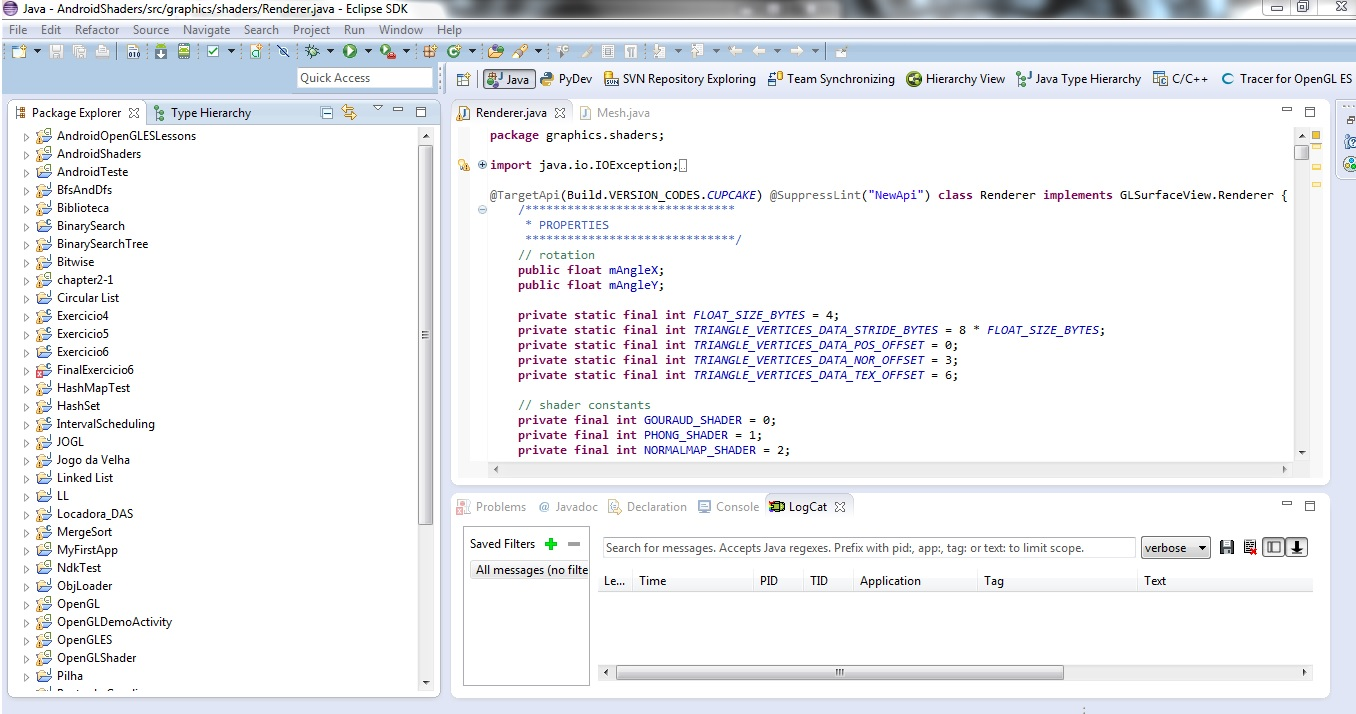
\includegraphics[keepaspectratio=true,scale=0.35]{figuras/eclipse.jpg}
	\caption{Ambiente de desenvolvimento \textit{Eclipse}}
	\label{eclipse}
	\end{figure}

	Além disso, também foi necessário instalar o \textit{Android NDK}, a fim de poder utilizar linguagem de código nativo C e acessar as extensões da \textit{OpenGL ES}. A biblioteca gráfica para sistemas embarcados \textit{OpenGL ES} já faz parte das ferramentas de desenvolvimento da plataforma \textit{Android}. 

\subsection{Plataforma \textit{iOS}}

	Para o desenvolvimento na plataforma \textit{iOS}, foi utilizada a ferramenta \textit{Xcode}. Segundo \cite{neub2013}, um novo projeto no \textit{Xcode} já vem com todos os arquivos e configurações necessários para o desenvolvimento de um aplicativo (Figura \ref{xcode}).  Esta ferramenta também possui um módulo chamado \textit{Instruments}, que analisa o comportamento interno de um aplicativo graficamente e numericamente, sendo possível monitorar diversas métricas.  

	\begin{figure}[ht]
	\centering
		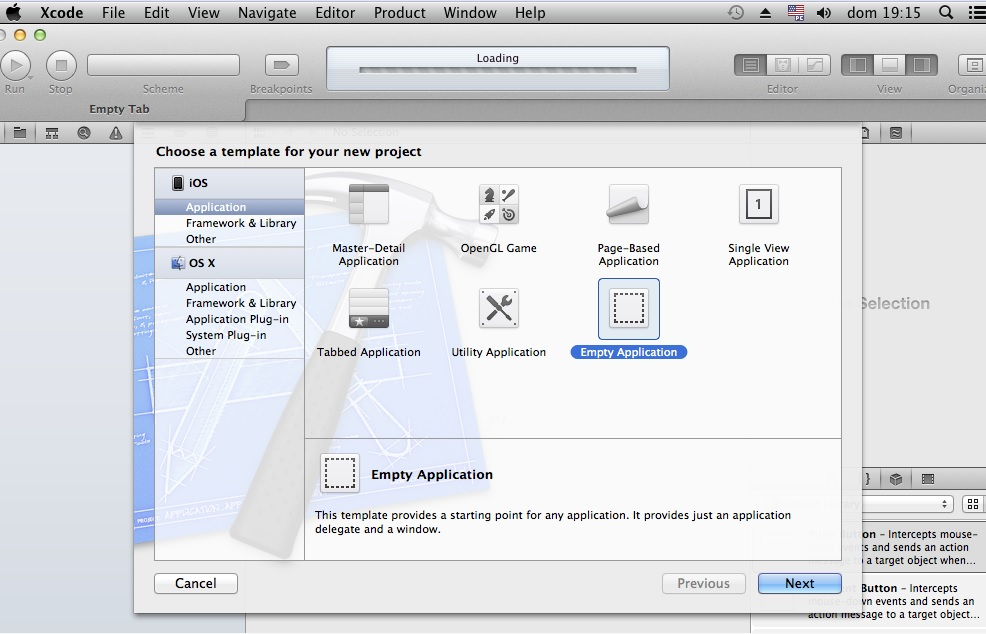
\includegraphics[keepaspectratio=true,scale=0.5]{figuras/xcode.jpg}
	\caption{Novo projeto de um aplicativo na ferramenta \textit{Xcode}}
	\label{xcode}
	\end{figure}

\subsection{Modelagem dos Objetos Tridimensionais}

 A fim de variar a contagem poligonal dos objetos tridimensionais, foi utilizada a ferramenta de modelagem tridimensional \textit{open source} chamada Blender\footnote{\textit{http://www.blender.org/}}, a qual está ilustrada na Figura \ref{blender}. Ela também permite modificar o número de polígonos de um modelo tridimensional por meio de modificadores chamados \textit{Decimate} e \textit{Subdivision Surface} (usados para diminuir e aumentar a contagem poligonal, respectivamente). 

	\begin{figure}[ht]
	\centering
		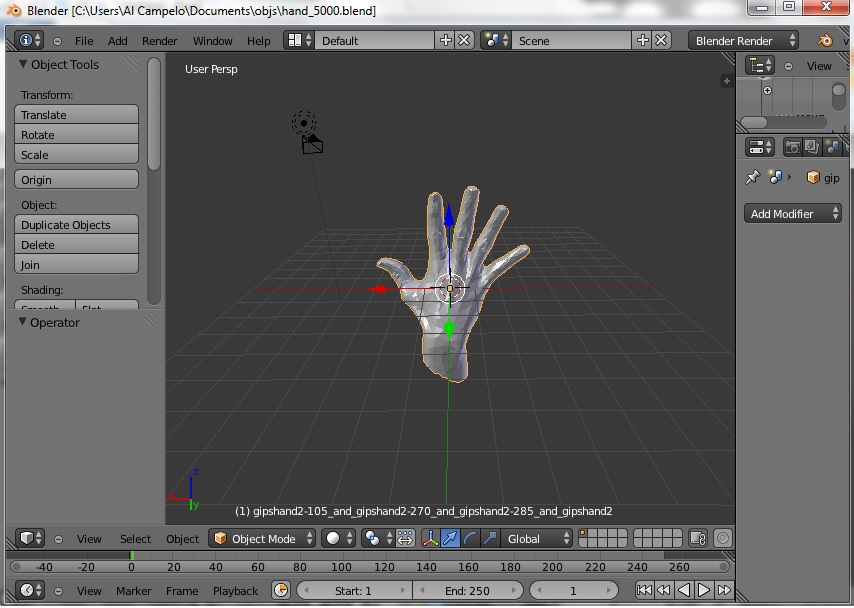
\includegraphics[keepaspectratio=true,scale=0.6]{figuras/blender.jpg}
	\caption{Ferramenta de modelagem tridimensional}
	\label{blender}
	\end{figure}

\subsection{Coleta de Medições}
\label{medicoes}

	Para a coleta das medições quanto a todo o processo de renderização, na plataforma \textit{Android}, foi utilizada uma extensão da \textit{OpenGL ES}. Esta extensão se chama \texttt{GL\_EXT\_disjoint\_timer\_query}\footnote{\textit{http://www.khronos.org/registry/gles/}}, e dentre os dispositivos utilizados neste trabalho, só está disponível para o \textit{Nexus 4} a partir da versão de Android 4.4 (\textit{KitKat}). A fim de utilizar esta extensão, foi necessário instalar e configurar o NDK (\textit{Native Development Kit}) e alterar o \textit{header} da versão da \textit{OpenGL ES} utilizada, adicionando as linhas de código relacionadas à extensão almejada. Assim, foi possível utilizar as novas funções desta extensão pegando os seus endereços por meio do comando \texttt{eglGetProcAddress} (disponível por meio da API EGL que faz o interfaceamento entre a \textit{OpenGL ES} e o sistema operacional). A integração entre o código em linguagem C e o código em Java foi feita por meio da JNI (\textit{Java Native Interface}). 

	A fim de realizar a mesma medição na plataforma \textit{iOS}, utilizou-se (como mostra a Figura \ref{instruments}) o módulo \textit{Instruments} da ferramenta \textit{Xcode}.

	\begin{figure}[ht]
	\centering
		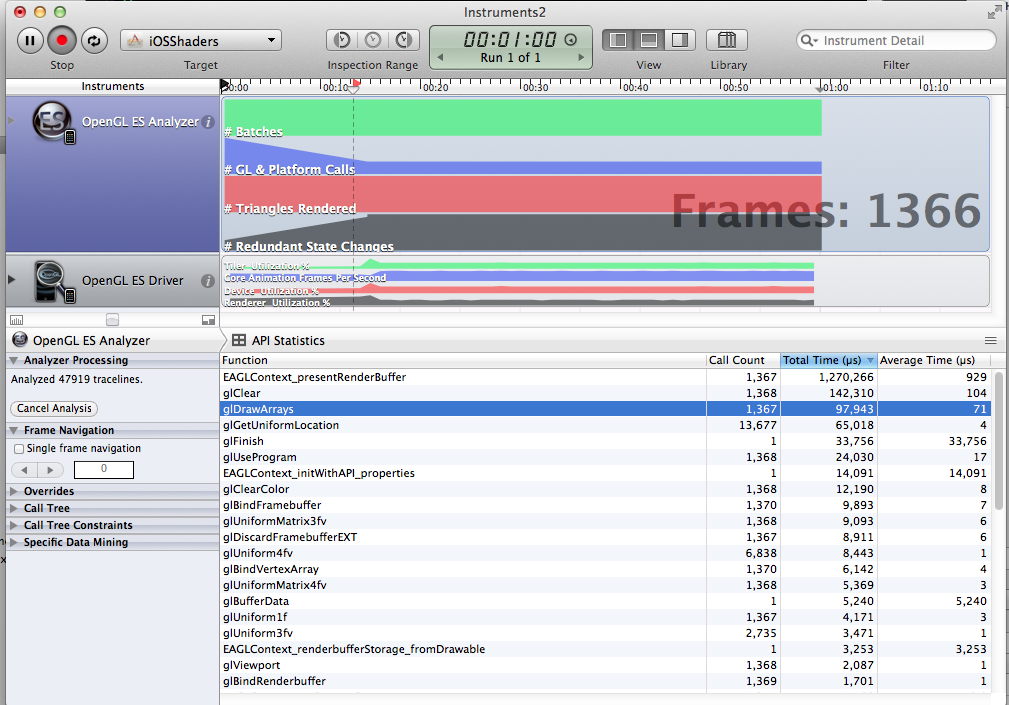
\includegraphics[keepaspectratio=true,scale=0.3]{figuras/analyzer_opengles.png}
	\caption{Analisador de \textit{OpenGL ES}}
	\label{instruments}
	\end{figure}


	Para a coleta das medições específicas do \textit{vertex} e \textit{fragment shaders} foi utilizada a ferramenta \textit{Adreno Profiler}, pois os celulares com plataforma \textit{Android} utilizados possuem a GPU \textit{Adreno}. Quanto à plataforma \textit{iOS}, não é possível coletar estas medições. 

	A \textit{Adreno Profiler} é uma ferramenta que foca na otimização gráfica para celulares que possuem GPU \textit{Adreno} (fabricada pela empresa \textit{Qualcomm}). De acordo com  \cite{adp}, a ferramenta provê suporte para \textit{Android} e \textit{Windows RT} (variação do sistema operacional \textit{Windows} 8  e projetada para \textit{devices} móveis), permitindo a otimização, análise por quadros e visualização de desempenho em tempo real. No dispositivo \textit{Nexus 4} ela só é suportada com o \textit{Android} até a versão 4.3 (não suporta o \textit{KitKat}).

	Como pode ser visto na Figura \ref{adrenoProfiler}, a ferramenta possui um módulo de análise dos \textit{vertex} e \textit{fragment} \textit{shaders}, sendo possível editá-los e analisar os resultados da compilação em tempo real, além de também gerar outras estatísticas.  

	\begin{figure}[ht]
	\centering
		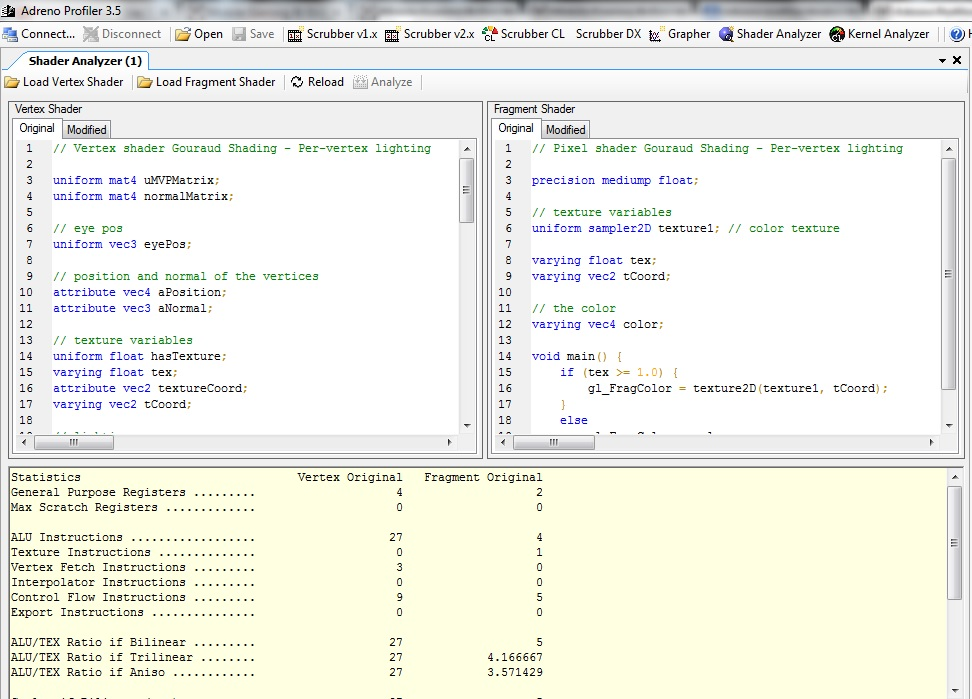
\includegraphics[keepaspectratio=true,scale=0.4]{figuras/shader_analyzer.jpg}
	\caption{Ferramenta \textit{Adreno Profiler}: analisador de \textit{shaders}}
	\label{adrenoProfiler}
	\end{figure}

	O módulo gráfico desta ferramenta permite analisar algumas métricas, relacionadas ao \textit{vertex} e \textit{fragment shaders}, conforme ilustrado na Figura \ref{graph}, em que um gráfico é plotado em tempo de execução. Além disso, ela também exporta os resultados no formato CSV (\textit{Comma-Separated Values}), que consiste em um arquivo de texto que armazena valores tabelados separados por um delimitador (vírgula ou quebra de linha). O último módulo é o chamado \textit{Scrubber}, que provê informações detalhadas quanto ao rastreamento de uma chamada de função. 

	\begin{figure}[ht]
	\centering
		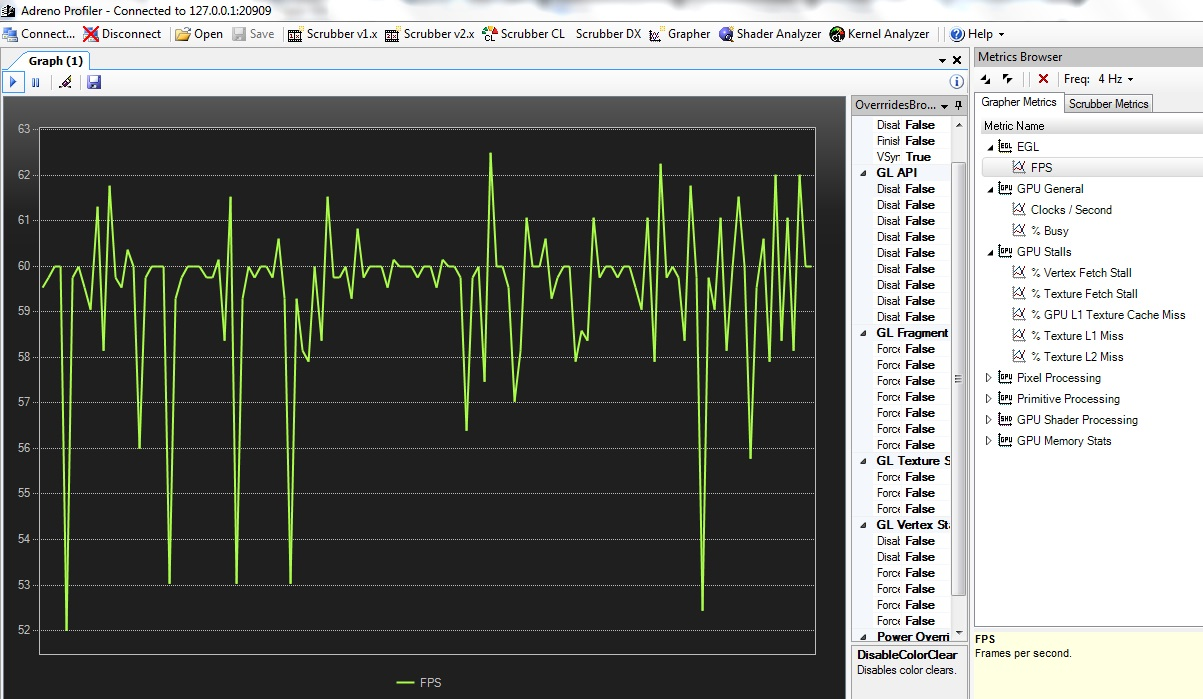
\includegraphics[keepaspectratio=true,scale=0.35]{figuras/graph.jpg}
	\caption{Ferramenta \textit{Adreno Profiler}: visualização de métrica quadros por segundo}
	\label{graph}
	\end{figure}

\subsection{Automatização de Cálculo e Plotagem}

	Para a automatização da plotagem dos gráficos e aplicação do método dos mínimos quadrados (descrito na Seção \ref{metminqua}) utilizou-se a linguagem de programação Python\footnote{\textit{http://www.python.org.br/}} versão 2.7.3, juntamente com os pacotes  \textit{matplotlib}\footnote{\textit{http://www.matplotlib.org/}} e  \textit{numpy}\footnote{\textit{http://www.numpy.org/}}. 

\subsection{Controle de Versionamento}

	O controle de versionamento do código foi feito por meio do sistema de controle de versão Git \footnote{\textit{http://git-scm.com/}} utilizando o \textit{forge} GitHub \footnote{\textit{https://github.com/}}. Foram criados repositórios tanto para as implementações em \textit{Android} e \textit{iOS}, quanto para a automatização da análise da complexidade assintótica.

\section{Implementação na Plataforma \textit{Android}} 
\label{imp}

	 A fim de tornar possível a realização da análise da complexidade algorítmica experimentalmente, primeiramente focou-se na implementação dos \textit{shaders} para plataforma \textit{Android} utilizando a biblioteca \textit{OpenGL ES}. Foi utilizado  o paradigma de orientação a objetos, em que o diagrama de classes (Figura \ref{class_diagram}) mostra como o código foi estruturado. Este diagrama mostra um conjunto de classes e seus relacionamentos, sendo o diagrama central da modelagem orientada a objetos. 

	\begin{figure}[ht]
	\centering
		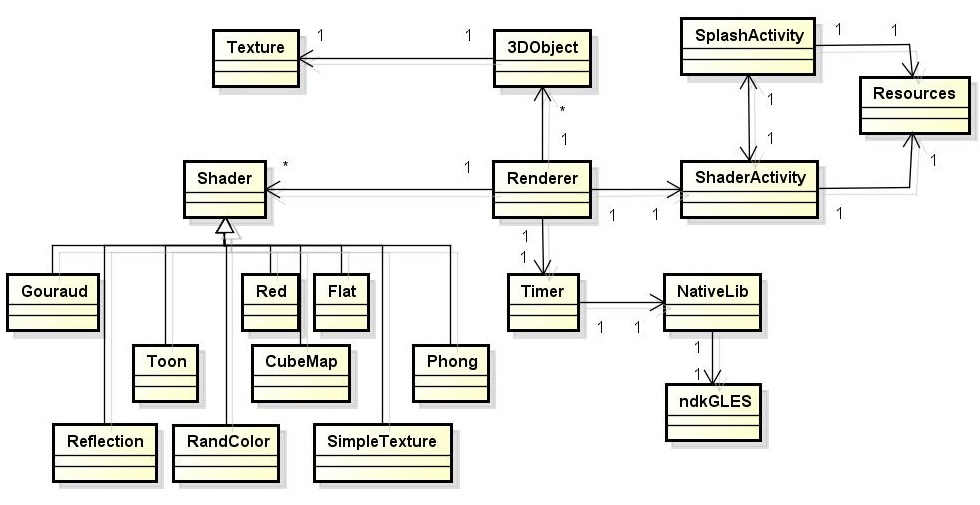
\includegraphics[keepaspectratio=true,scale=0.5]{figuras/class_diagram.jpg}
	\caption{Diagrama de Classe da Implementação em \textit{Android}}
	\label{class_diagram}
	\end{figure}

\subsection{Tela de \textit{Front-end}}

	\begin{figure}[ht]
	\centering
		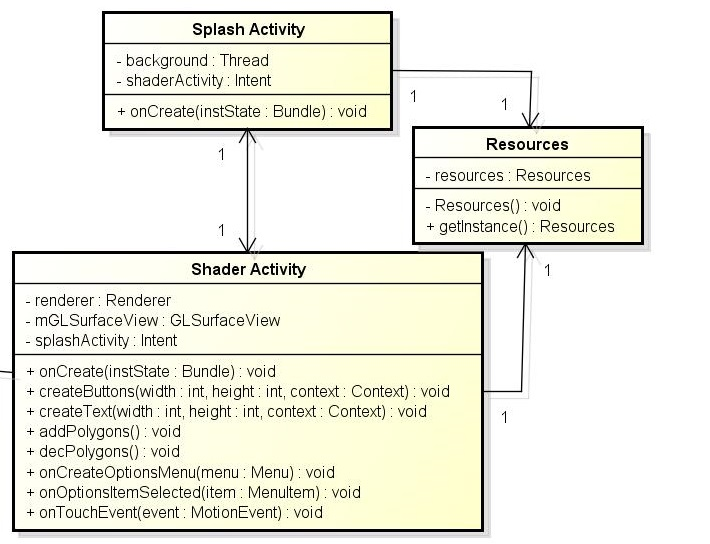
\includegraphics[keepaspectratio=true,scale=0.5]{figuras/shader_splash.jpg}
	\caption{Detalhamento das classes \textit{Shader Activity}, \textit{Splash Activity} e \textit{Resources}}
	\label{shader_splash}
	\end{figure}

	A tela de \textit{front-end} é responsável pela interação com o usuário, repassando as informações de entrada para o \textit{back-end}. E de acordo com \cite{androidsdkmanager}, a plataforma \textit{Android} utiliza o termo \textit{Activity} para descrever esta tela de \textit{front-end} da aplicação. Ela possui elementos de \textit{design} como texto, botões, gráficos, entre outros. No contexto deste trabalho, há duas classes \textit{Activity} (Figura \ref{shader_splash}), a \textit{Shader} e a \textit{Splash}. 

	A \textit{Splash Activity} (Figura  \ref{splash_act}) é responsável pela visualização da tela de \textit{loading} enquanto são carregados os recursos necessários para o programa (como a leitura dos modelos tridimensionais em formato \textit{obj} e das imagens usadas para texturização) por meio do uso de uma \textit{thread}. Estes recursos são gerenciados pela classe \textit{Resources}, que utiliza o padrão de projeto \textit{Singleton}, que garante a existência de apenas uma instância da classe, que será acessada posteriormente.

	\begin{figure}[ht]
	\centering
		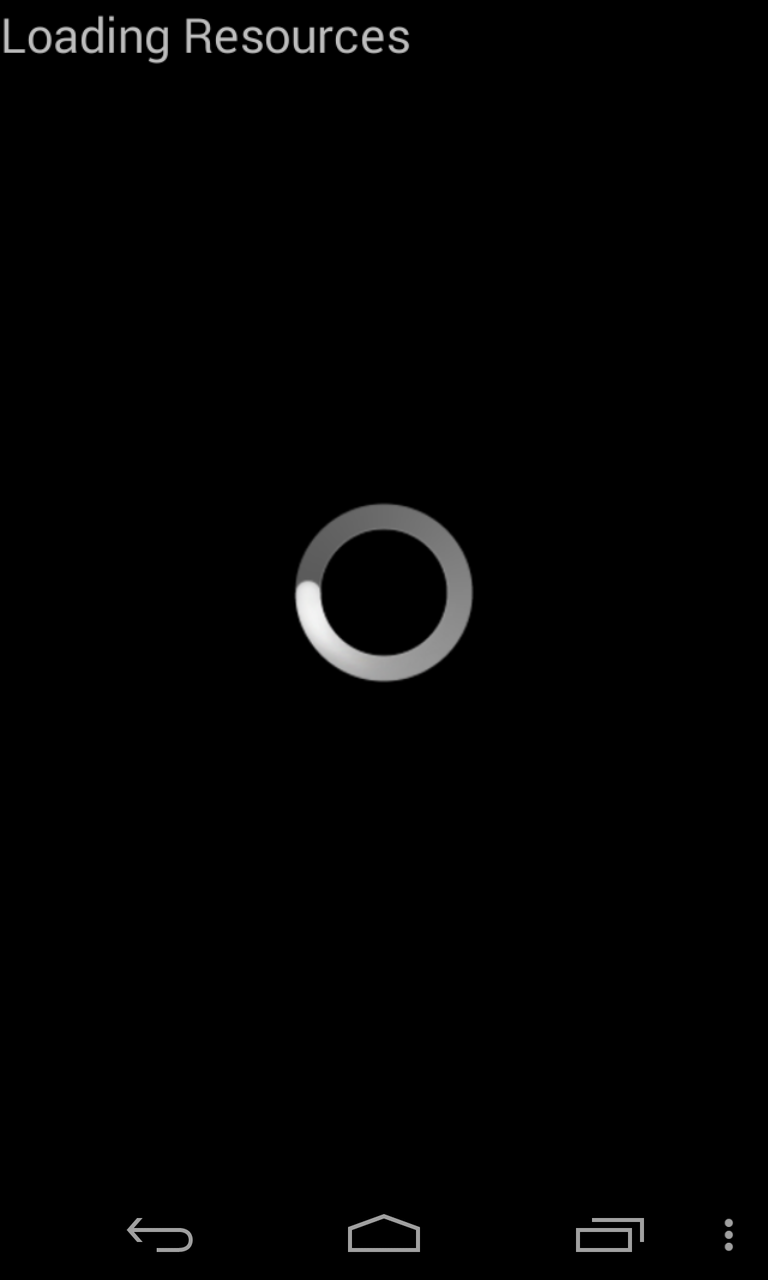
\includegraphics[keepaspectratio=true,scale=0.2]{figuras/splash_act.png}
	\caption{Tela da \textit{Splash Activity}}
	\label{splash_act}
	\end{figure}

	A \textit{Shader Activity} (Figura  \ref{shader_act}) é responsável pela  instanciação da classe \textit{Renderer}, que renderiza os gráficos tridimensionais utilizando a biblioteca \textit{OpenGL ES}. Além disso, ela controla os eventos de \textit{touch}, que permitem escalar e mover o objeto, além de disponibilizar o menu que troca de \textit{shader}, os botões que aumentam ou diminuem o número de polígonos, a informação do tempo de renderização e a da quantidade de polígonos. O aumento do número de polígonos é realizado através da troca de objetos que possuem arquivos \textit{obj} diferentes, que já foram carregados pela \textit{Splash Activity}. 

	\begin{figure}[ht]
	\centering
		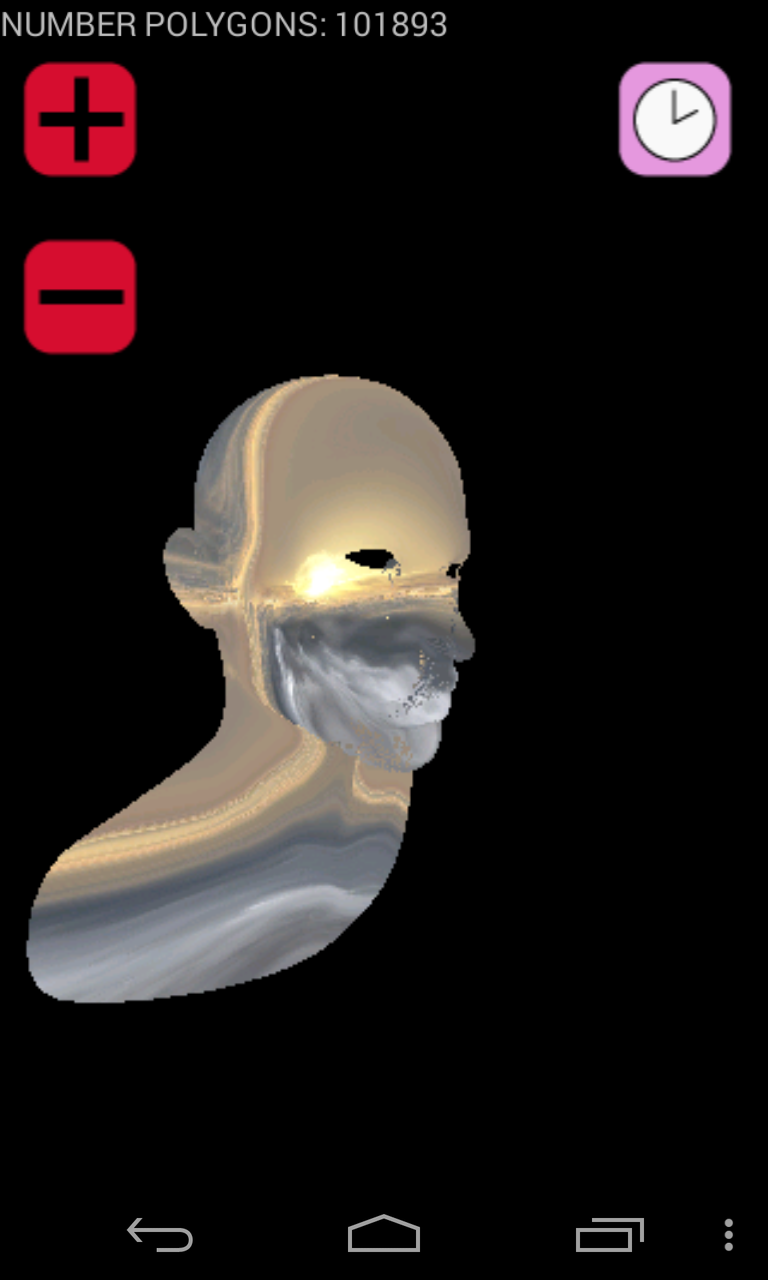
\includegraphics[keepaspectratio=true,scale=0.2]{figuras/shader_act.png}
	\caption{Tela da \textit{Shader Activity}}
	\label{shader_act}
	\end{figure}

	Devido à limitação de memória do dispositivo móvel e os vários objetos com diferentes números de polígonos, não é possível carregar todos de uma só vez. Assim, foi necessário delimitar esta quantidade de objetos simultâneos: uma vez atingido o valor limítrofe (tanto adicionando, quanto decrementando), volta-se novamente para a \textit{Splash Activity}, a fim de carregar os novos objetos e retornar para a \textit{Shader Activity}, onde serão renderizados.

\subsection{Objeto Tridimensional}   

	\begin{figure}[ht]
	\centering
		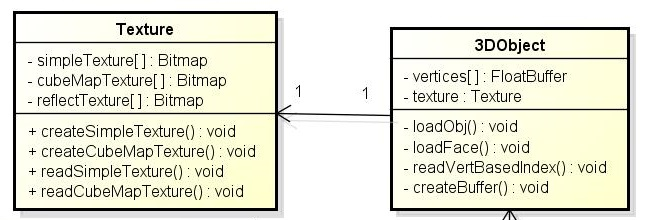
\includegraphics[keepaspectratio=true,scale=0.6]{figuras/object_texture.jpg}
	\caption{Detalhamento das classes \textit{3DObject} e \textit{Texture}}
	\label{object_texture}
	\end{figure}

	O objeto tridimensional foi representado pela composição das classes \textit{3DObject} e \textit{Texture}. A classe \textit{3DObject}, mostrada na Figura \ref{object_texture}, é responsável por ler e interpretar os arquivos \textit{obj}  (descritos no Anexo \ref{formatobj}), criados por meio da ferramenta \textit{Blender}.

	Após a leitura e interpretação do arquivo \textit{obj} foi gerado um \textit{buffer} para armazenar os vértices de posição, normal e textura na ordem em que eles são renderizados. Neste \textit{buffer} cada coordenada relacionada a um vértice (posição, normal e textura) é armazenada alternadamente, como mostra a Figura \ref{buffer}.

	\begin{figure}[ht]
	\centering
		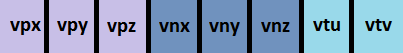
\includegraphics[keepaspectratio=true,scale=1.0]{figuras/buffer.png}
	\caption{Ordem das coordenadas de posição, normal e textura para um vértice}
	\label{buffer}
	\end{figure}

	A classe \textit{Texture} gera as texturas utilizadas pelos \textit{shaders} \textit{SimpleTexture}, \textit{CubeMap} e \textit{Reflection}, a partir de imagens. Estas imagens são criadas para cada modelo tridimensional, utilizando a técnica de \textit{UV Mapping}, na qual mapeiam-se as coordenadas de textura para uma imagem (Figura \ref{uvmap}). Como a orientação do eixo de coordenas $y$ da ferramenta \textit{Blender} é diferente da \textit{OpenG ES}, é necessário refletir a imagem neste eixo para corrigir o mapeamento.

	Para gerar uma textura simples, primeiramente gera-se um objeto de textura utilizando a função \texttt{glGenTextures()}, depois vincula-se esta textura ao objeto com a função \texttt{glBindTexture()} e carrega-se a imagem por meio da função \texttt{texImage2D()}.  Para as texturas do \textit{CubeMap} e \textit{Reflection}, faz-se a mesma coisa, exceto que a função \texttt{texImage2D()} é feita seis vezes, uma vez que cada textura representa uma face de um cubo. 

	\begin{figure}[ht]
	\centering
		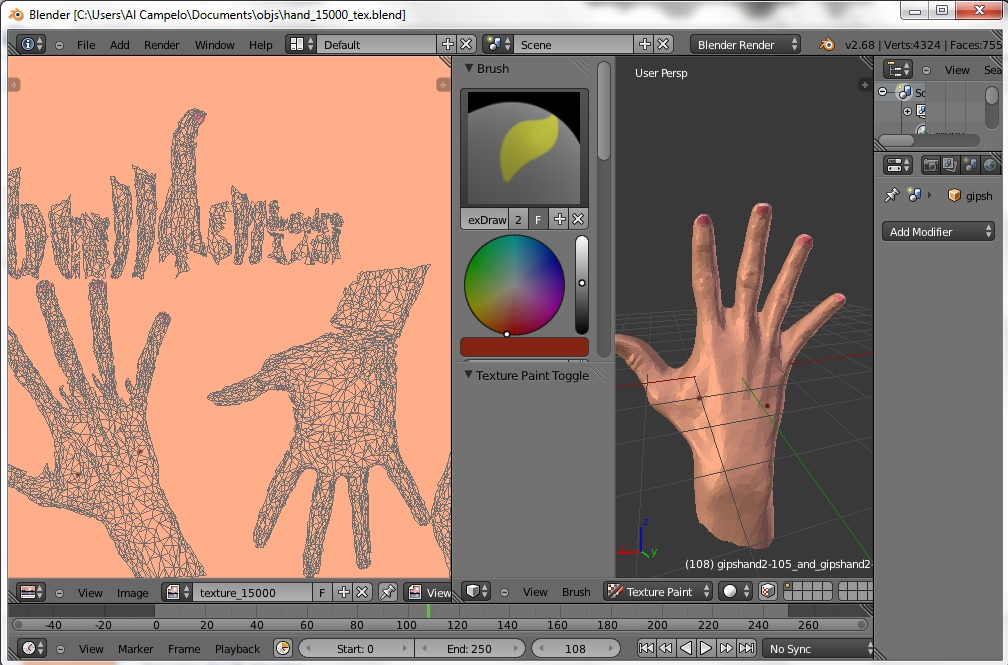
\includegraphics[keepaspectratio=true,scale=0.6]{figuras/uvmap.jpg}
	\caption{Técnica de mapeamento de textura utilizada para cada modelo 3D}
	\label{uvmap}
	\end{figure}

	A Figura  \ref{texture_uvmap} apresenta a imagem resultante da técnica de mapeamento realizada.

	\begin{figure}[ht]
	\centering
		
\includegraphics[keepaspectratio=true,scale=0.2]{figuras/texture_uvmap.jpg}
	\caption{Textura gerada a partir da técnica de mapeamento}
	\label{texture_uvmap}
	\end{figure}

\subsection{Cálculo do Tempo de Renderização}      

	\begin{figure}[ht]
	\centering
		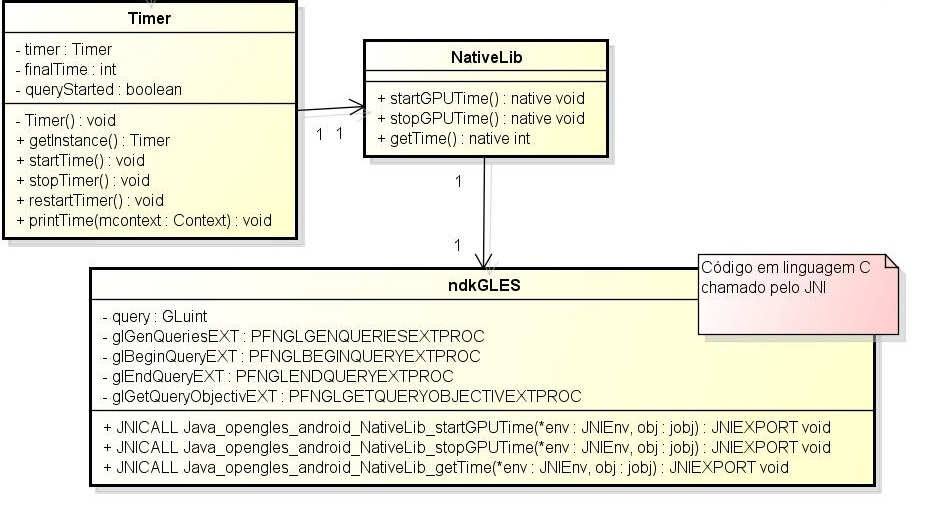
\includegraphics[keepaspectratio=true,scale=0.6]{figuras/timer_nativelib.jpg}
	\caption{Detalhamento das classes \textit{Timer} e \textit{NativeLib}}
	\label{timer_nativelib}
	\end{figure}

	A Figura \ref{timer_nativelib} detalha a classe \textit{Timer}, que realiza a média de dez medições do tempo de renderização (em nanosegundos) para cada objeto tridimensional. Cada medição é feita utilizando a linguagem C e a extensão da \textit{OpenGL ES}, citada na Seção \ref{gpu}, chamada \texttt{GL\_EXT\_disjoint\_timer\_query}.  A integração entre o código em linguagem C e o código em Java é feita por meio da classe \textit{NativeLib}. Caso a extensão não esteja disponível para o dispositivo, um alerta é emitido.

\subsection{Renderização}    

	\begin{figure}[ht!]
	\centering
		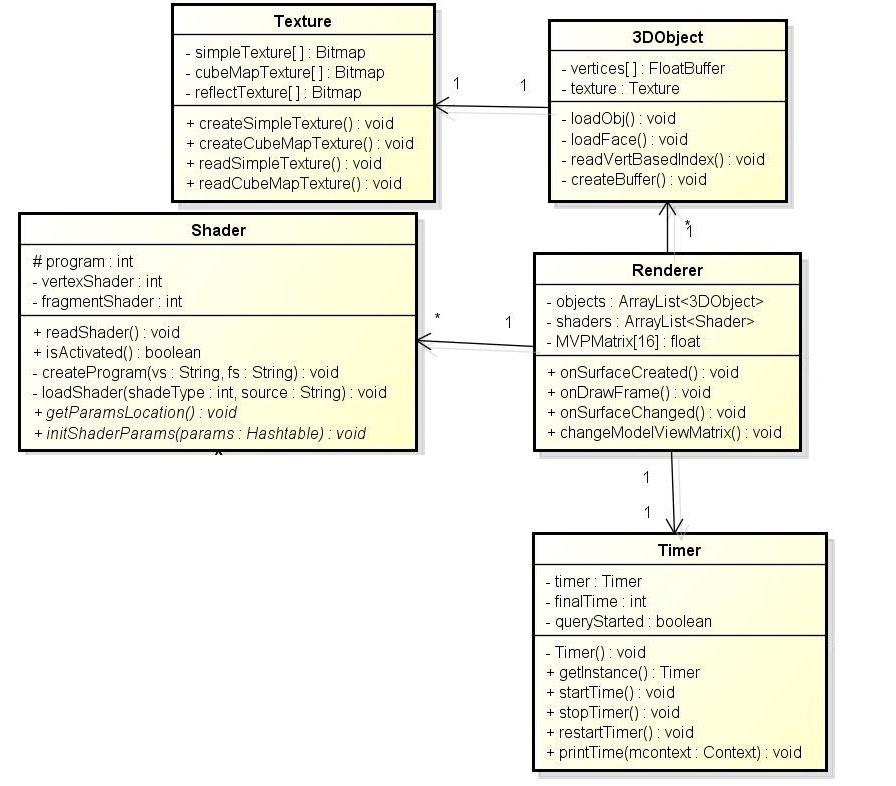
\includegraphics[keepaspectratio=true,scale=0.6]{figuras/renderer.jpg}
	\caption{Detalhamento da classe \textit{Renderer}}
	\label{renderer}
	\end{figure}

	A Figura \ref{renderer} mostra a classe \textit{Renderer}, responsável pela renderização, que funciona como uma controladora, sendo o ponto principal  das chamadas provenientes da \textit{view} (\textit{ShaderActivity}) para as classes de \textit{model} (\textit{3DObject}, \textit{Shader} e \textit{Timer}). Ela implementa as funções da biblioteca \textit{OpenGL ES} \texttt{onSurfaceCreated()},  \texttt{onDrawFrame()} e \texttt{onSurfaceChanged()}. A primeira função é chamada apenas uma vez quando a \textit{view} da \textit{OpenGL ES} é instanciada, e é responsável por todas as configurações, como por exemplo, a criação de texturas. A segunda função é chamada em \textit{loop}, onde é feita a renderização por meio da função \texttt{glDrawArrays()}. 

\subsection{\textit{Shaders}}      

	\begin{figure}[ht]
	\centering
		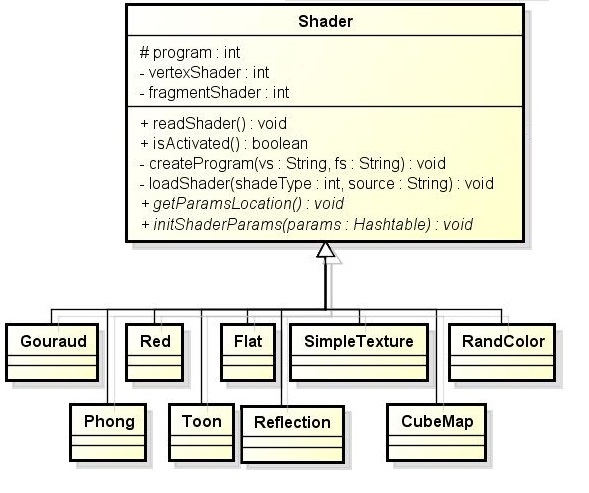
\includegraphics[keepaspectratio=true,scale=0.6]{figuras/shaders_diag.jpg}
	\caption{Detalhamento da classe \textit{Shader}}
	\label{shaders_diag}
	\end{figure}

	A classe \textit{Shader} (Figura \ref{shaders_diag}) é responsável por ler, fazer o \textit{attach} e o \textit{link} do \textit{ vertex} e do \textit{fragment shaders}. Além disso, ela possui os métodos abstratos \texttt{getParamsLocation()} e \texttt{initShaderParams(Hastable params)}. O primeiro método faz o armazenamento da localização de cada variável especificada dentro do \textit{shader}, já o segundo método inicializa estas variáveis por meio de um \textit{hash} que é passado como um parâmetro pela classe \textit{Renderer}. Assim, todos os \textit{shaders} implementados herdam da classe \textit{Shader} e implementam seus métodos abstratos. Estes \textit{shaders} podem ser vistos na Figura \ref{shaders_impl}.  

	\begin{figure}[ht]
	\centering
		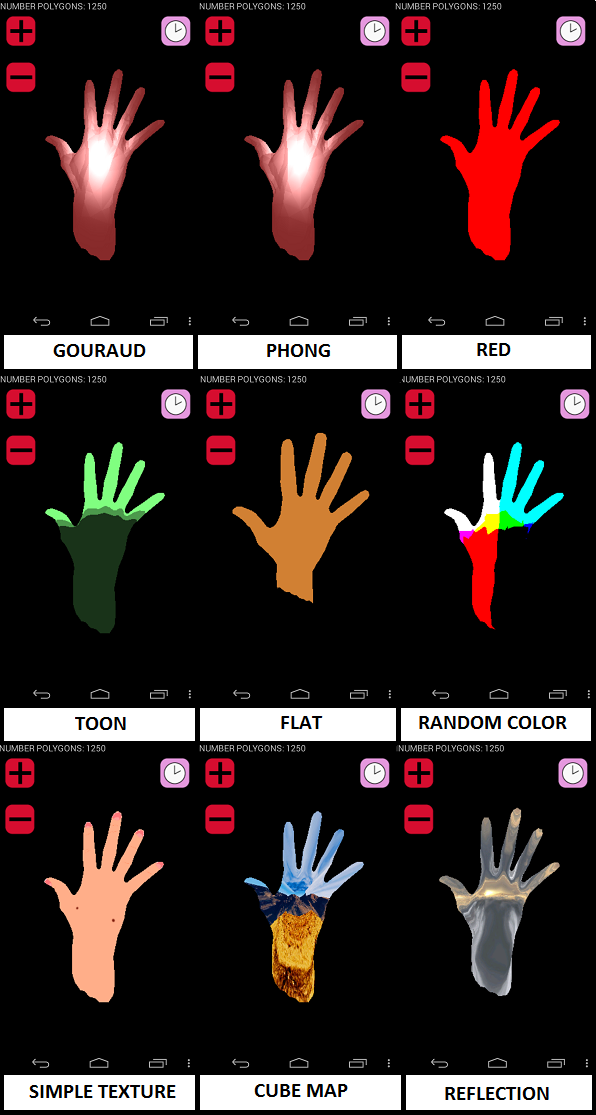
\includegraphics[keepaspectratio=true,scale=0.7]{figuras/shaders_impl.png}
	\caption{\textit{Shaders} Implementados}
	\label{shaders_impl}
	\end{figure}

	A seguir, alguns dos \textit{shaders} implementados serão apresentados.

\subsubsection{\textit{Phong Shader}}

	O \textit{vertex} e \textit{fragment shaders} do \textit{phong shading} implementam a técnica descrita na Seção \ref{flatgouphon}, em que primeiramente interpolam-se os valores dos vetores normais das primitivas e então computam-se os cálculos de luz para cada fragmento, utilizando os vetores normais interpolados. O Código \ref{codphongvs} e o Código \ref{codphongfs} mostram as definições do \textit{vertex} e \textit{fragment shaders}, respectivamente, os quais utilizam as variáveis que definem as propriedades do material.  

	\lstinputlisting[language=C, label = {codphongvs}, caption = {\textit{Phong Shader}:  \textit{vertex shader}}]{codigos/phong_vs.txt}

	\lstinputlisting[language=C, caption =  {\textit{Phong Shader}:  \textit{fragment shader}}, label = {codphongfs}  ]{codigos/phong_ps.txt}

\subsubsection{\textit{Gouraud Shader}}

	O \textit{Gouraud Shader}, assim com o \textit{Phong Shader}, também implementa a técnica descrita na Seção \ref{flatgouphon}, porém os cálculos de luz e da cor são feitos no \textit{vertex shader} para serem interpolados e passados para o \textit{fragment shader}, como mostram o Código \ref{codgouraudvs} e o Código \ref{codgouraudfs}. 

	\lstinputlisting[language=C, label = {codgouraudvs}, caption = {\textit{Gouraud Shader}:  \textit{vertex shader}}]{codigos/gouraud_vs.txt}

	\lstinputlisting[language=C, caption =  {\textit{Gouraud Shader}:  \textit{fragment shader}}, label = {codgouraudfs}  ]{codigos/gouraud_ps.txt}
	
\subsubsection{\textit{Red Shader}}
	
	O \textit{shader} que define a cor do fragmento como vermelha é muito simples:  o \textit{vertex shader} apenas estabelece que a posição do vértice  se dá pela multiplicação da matriz de projeção, visualização e modelagem pela coordenada (variável \texttt{aPosition}) como é mostrada no Código \ref{codredvs}. 
	
	\lstinputlisting[language=C, caption = {\textit{Red Shader}:  \textit{vertex shader}}, label = {codredvs}]{codigos/red_vs.txt}

	Já o seu \textit{fragment shader} (Código \ref{codredfs}) estabelece que todo fragmento possui a cor vermelha, por meio da variável pré-definida \texttt{gl\_FragColor}.
	
	\lstinputlisting[language=C, caption = {\textit{Red Shader}:  \textit{fragment shader}}, label = {codredfs}]{codigos/red_ps.txt}

\subsubsection{\textit{Toon Shader}}

	O  \textit{toon shader} calcula a intensidade da luz por vértice para escolher uma das cores pré-definidas, como apresentado na Seção \ref{teoria}. O Código  \ref{codtoonvs} mostra o cálculo da intensidade da luz por vértice, utilizando primeiro a direção da luz (definida como uma variável \texttt{uniform} passada pelo programa) para depois fazer o produto escalar entre ela e o vetor normal (cálculo da intensidade da luz).  

	\lstinputlisting[language=C,label = {codtoonvs}, caption = {\textit{Toon Shader}:  \textit{vertex shader}} ]{codigos/toon_vs.txt}

	A variável \textit{intensity}, do tipo \textit{varying}, é passada do \textit{vertex shader} para o \textit{fragment shader}, a fim de determinar qual das três cores será escolhida (Código \ref{codtoonfs}). 
  
 	\lstinputlisting[language=C, caption = {\textit{Toon Shader}:  \textit{fragment shader}}, label = {codtoonfs} ]{codigos/toon_ps.txt}

\subsubsection{\textit{Flat Shader}}

	A ideia do \textit{Flat Shader} é tornar um modelo tridimensional em bidimensional, achatado. Para isto, a coordenada $z$ deve ser definida como zero, como é mostrado no Código \ref{codflatvs}. O \textit{fragment shader} (Código  Código \ref{codflatfs}) apenas define uma cor para o fragmento (Código \ref{codflatfs}).

	\lstinputlisting[language=C,label = {codflatvs}, caption = {\textit{Flat Shader}:  \textit{vertex shader}} ]{codigos/flat_vs.txt}

	\lstinputlisting[language=C, caption = {\textit{Flat Shader}:  \textit{fragment shader}}, label = {codflatfs} ]{codigos/flat_ps.txt}

\subsubsection{\textit{Random Color Shader}}

	O \textit{Random Color Shader} determina a cor do fragmento, baseando-se em um cálculo matemático, que determina a cor final aleatoriamente. Este cálculo da cor é feito no \textit{vertex shader} (Código \ref{codrandvs}) e o valor resultante é passado para o \textit{fragment shader}, por meio da variável \textit{color} do tipo \textit{varying}. Cada componente da cor é calculada passando uma coordenada ($x$, $y$ ou $z$) para a função \texttt{random(vec2 v)}, que retorna um valor aleatório para a componente da cor, baseando-se nesta coordenada. O Código \ref{codrandfs} apenas determina a cor do fragmento, calculada pelo \textit{vertex shader}.

	\lstinputlisting[language=C,label = {codrandvs}, caption = {\textit{Random Color Shader}:  \textit{vertex shader}} ]{codigos/randcolor_vs.txt}
 
	\lstinputlisting[language=C, caption = {\textit{Random Color Shader}:  \textit{fragment shader}}, label = {codrandfs} ]{codigos/randcolor_ps.txt}

\subsubsection{\textit{Simple Texture Shader}}

	O \textit{vertex shader} do \textit{simple texture shading} primeiramente armazena as coordenadas de textura numa variável do tipo \textit{varying} (Código \ref{codtexvs}), e as repassa para o \textit{fragment shader}, além de também definir a posição do vértice.  

	\lstinputlisting[language=C, caption =  {\textit{Simple Texture Shader}:  \textit{vertex shader}}, label = {codtexvs} ]{codigos/simple_tex_vs.txt}

	No Código \ref{codtexfs}, o \textit{fragment shader}, por sua vez, utiliza a textura passada pelo programa e aplica a coordenada de textura, repassada pelo \textit{vertex shader}, no fragmento por meio da função \texttt{texture2D()} da GLSL.

	\lstinputlisting[language=C, caption =  {\textit{Simple Texture Shader}:  \textit{fragment shader}}, label = {codtexfs} ]{codigos/simple_tex_ps.txt}

\subsubsection{\textit{CubeMap Shader}}	

	 O \textit{vertex shader} do \textit{CubeMap Shader} é simples e só define a posição do vértice (Código \ref{codcubemapvs}). 

	\lstinputlisting[language=C, caption =  {\textit{CubeMap Shader}:  \textit{vertex shader}}, label = {codcubemapvs} ]{codigos/cubemap_vs.txt}

	O  \textit{fragment shader} (Código \ref{codcubemapps}), por sua vez, utiliza a função \texttt{textureCube( samplercube s, vec3 coord)} da GLSL, que recebe como parâmetros o vetor normal e a textura a ser mapeada. 

	\lstinputlisting[language=C, caption =  {\textit{CubeMap Shader}:  \textit{fragment shader}}, label = {codcubemapps} ]{codigos/cubemap_ps.txt}
	
\subsubsection{\textit{Reflection Shader}}

	O \textit{Reflection Shader} implementa a técnica descrita na Seção \ref{ref_t}. O seu \textit{vertex shader} é responsável por indicar que a posição do vértice se dá pela multiplicação da coordenada (variável \texttt{vec4 aPosition}) pela matriz de projeção, visualização e modelagem, como é mostrado no Código \ref{codreflvs}. Além disso, no \textit{vertex shader} são declarados dois vetores do tipo \textit{varying} (que passa o valor da variável ao \textit{fragment shader}) que estão relacionados com o vetor de direção da câmera e o vetor normal. 

	\lstinputlisting[language=C, caption = {\textit{Reflection Shader}:  \textit{vertex shader}}, label = {codreflvs}]{codigos/reflection_vs.txt}

	No \textit{fragment shader}, a normal e o vetor de direção da câmera são utilizados para encontrar o vetor da direção da reflexão através da utilização da função \texttt{reflect}. O vetor da direção da reflexão é utilizado na função \texttt{textureCube(samplercube s, vec3 coord)} (Código \ref{codreflfs}), em que determina-se a cor do fragmento, baseando-se nesta direção e em uma imagem. 

	\lstinputlisting[language=C, caption = {\textit{Reflection Shader}:  \textit{fragment shader}}, label = {codreflfs}]{codigos/reflection_ps.txt}

\section{Implementação na Plataforma \textit{iOS}} 

	A estrutura do programa portado para a plataforma \textit{iOS} é similar à feita para plataforma \textit{Android}, como mostra a Figura \ref{ios_diag}. Segundo \cite{neub2013}, o desenvolvimento para plataforma \textit{iOS} segue o padrão MVC (\textit{Model-View-Controller}), que é um padrão arquitetural. A classe (\textit{RendererViewController}) é a controladora responsável pela integração entre as classes \textit{Shader}, \textit{3DObject} e a a classe de visualização \textit{RendererView}. É na controladora que são feitas as principais chamadas da \textit{OpenGL ES}. A classe \textit{3DObject} faz a interpretação do arquivo \textit{obj} para o formato aceito pela \textit{OpenGL ES} e a classe \textit{Shader}, assim como na plataforma \textit{Android}, é responsável por ler, fazer o \textit{attach} e o \textit{link} do \textit{ vertex} e do \textit{fragment shaders}. 

	\begin{figure}[ht]
	\centering
		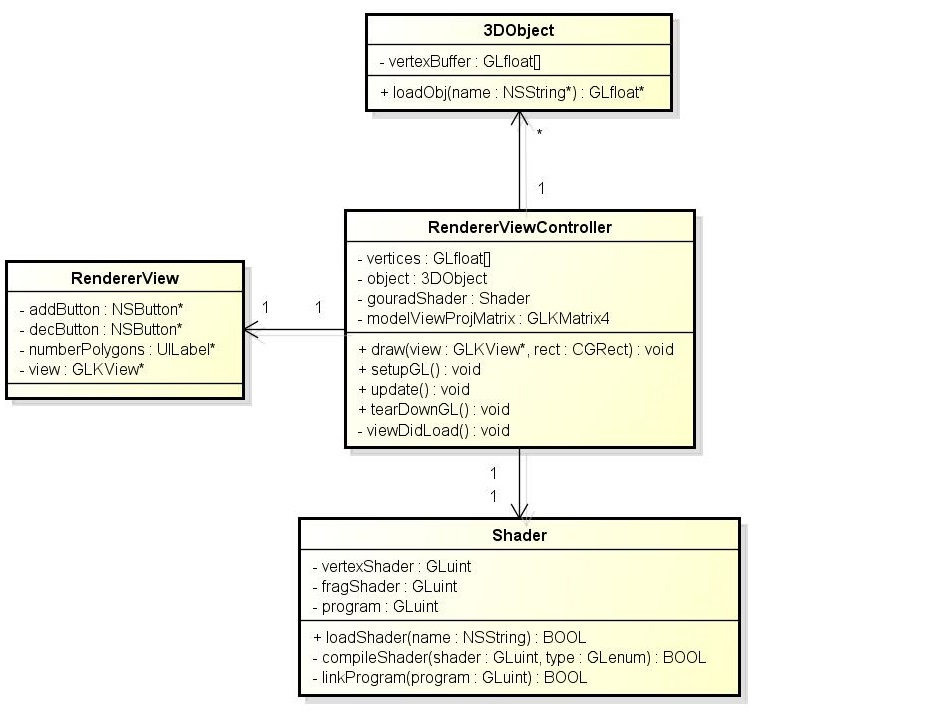
\includegraphics[keepaspectratio=true,scale=0.6]{figuras/ios_class_diagram.jpg}
	\caption{Diagrama de Classes da Implementação em \textit{iOS}}
	\label{ios_diag}
	\end{figure}

	Assim, escolheu-se um \textit{shader}, no caso o \textit{Gouraud Shader}, para ser implementado e posteriormente realizar as comparações entre os diferentes dispositivos e plataformas. O resultado da implementação pode ser visto na Figura \ref{gouraud_ios}.

	\begin{figure}[ht]
	\centering
		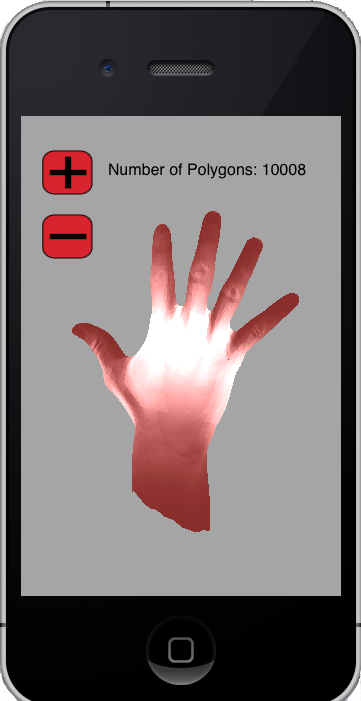
\includegraphics[keepaspectratio=true,scale=0.5]{figuras/gouraud_ios.png}
	\caption{\textit{Gouraud Shader} na plataforma \textit{iOS}}
	\label{gouraud_ios}
	\end{figure}

\section{Estimativa Experimental da Complexidade Algorítmica}

	A estimativa experimental da complexidade assintótica foi realizada através da coleta de diversas medições para cada modelo tridimensional (com diferentes quantidades de polígonos). Estas medidas foram plotadas em gráficos, cujas curvas foram ajustadas através do método dos mínimos quadrados (Seção \ref{metminqua}). Cada um destes processos é explicado a seguir.


\subsection{Medição do Processo de Renderização}
\label{gpu}

	A fim de estimar experimentalmente a análise da complexidade assintótica dos \textit{shaders} implementados, primeiro buscou-se coletar uma métrica relacionada ao tempo de renderização, que calcula o tempo necessário para processar o \textit{shader} como um todo. Por meio de pesquisa e consulta na documentação da \textit{OpenGL ES} para a plataforma \textit{Android}, conseguiu-se encontrar uma extensão desta biblioteca gráfica, explicada na Seção \ref{medicoes}, que permite contabilizar o tempo, em nanosegundos, necessário para realizar chamadas de \textit{OpenGL ES} específicas. Porém esta extensão só está disponível para alguns dispositivos e foi utilizada para medir o tempo de todo o processo de renderização realizado pela função \texttt{glDrawArrays()}.

	Para a plataforma \textit{iOS}, utilizou-se um módulo da ferramenta \textit{Xcode} também explicado na Seção \ref{medicoes}, que assim como a extensão da \textit{OpenGL ES}, consegue calcular o tempo da chamada da função \texttt{glDrawArrays()}, porém em microssegundos.  

	Assim, as medições do tempo do processo de renderização foram coletadas para o dispositivo \textit{Nexus 4}, \textit{iPhone 5s} e \textit{iPad Air}. A medição não foi feita para o dispositivo \textit{HTC One}, onde a extensão \texttt{GL\_EXT\_disjoint\_timer\_query} não está disponível.

\subsection{Medição do \textit{Vertex} e  \textit{Fragment Shaders}}

	Para a coleta de medições relacionadas ao \textit{vertex} e \textit{fragment} \textit{shaders}, utilizou-se a ferramenta \textit{Adreno Profiler}, mostrada na Seção \ref{medicoes}. As métricas escolhidas foram a de número de instruções por segundo por vértice e número de instruções por segundo por fragmento. Estas métricas foram coletadas para cada número específico de polígonos, sendo os resultados exportados no formato CSV. Porém, como esta ferramenta só pode ser utilizada em dispositivos com GPU Adreno, as medições foram realizadas apenas para os dispositivos \textit{Nexus 4} e \textit{HTC One} (para este último dispositivo, escolheu-se apenas o \textit{Gouraud Shader} para comparação). 

	A medição do \textit{vertex} e \textit{fragment shaders} não puderam ser feitas para a plataforma \textit{iOS}, pois o módulo \textit{Instruments} não disponibiliza nenhuma métrica relacionada.

\subsection{Plotagem}

	Após feitas as medições, foram plotados os gráficos tanto para todo o processo de renderização, quanto para o \textit{vertex} e \textit{fragment shaders}. O primeiro conjunto de gráficos está relacionado com o tempo em nanosegundos \textit{versus} a quantidade de polígonos, e o segundo, com o número de instruções por vértice (ou fragmento) \textit{versus} a quantidade de polígonos.

\subsection{Automatização dos Ajustes das Curvas}

	A fim de ajustar as curvas obtidas por meio das medições, e consequentemente estimar a complexidade assintótica, utilizou-se o método dos mínimos quadrados (Seção \ref{metminqua}) para funções lineares, quadráticas, cúbicas e exponenciais, calculando-se os respectivos erros, e determinando qual destas curvas melhor aproximava das medições. 

	 Para automatizar este cálculo do ajuste, foi feito um programa em Python que lê os arquivos CSV, computa a média das medições, plota os gráficos para o \textit{vertex} e \textit{fragment} \textit{shaders} e realiza os ajustes das curvas, calculando os erros associados e determinando o menor entre eles.  Este programa também pode ler as medições a partir de um arquivo de extensão .\textit{txt} e realizar os ajustes das curvas para todo o processo de renderização (utilizando a medição do tempo em nanosegundos). Este programa (\textit{script}) é executado por linha de comando, tendo como parâmetro o \textit{shader} desejado e qual medição utilizada (se a relacionada a cada tipo de \textit{shader} ou ao processo de renderização como um todo. Dois exemplos de linhas de comando podem ser vistos no Código \ref{linhacomando}). A primeira linha está relacionada com o cálculo para todo o processos de renderização, e a segunda, apenas para o \textit{vertex} e \textit{fragment shaders}.

	\lstinputlisting[language=C, numbers=none,label = {linhacomando}, caption = {Linhas de comando}]{codigos/linhacomando.txt}

	O programa foi estruturado de acordo com a Figura \ref{minquad_diag}, em que a classe \textit{ReadCSV} é responsável por ler os arquivos CSV e computar a média das métricas tanto para o \textit{vertex shader} como para o \textit{fragment shader}. A classe \textit{ReadTxt} é responsável por ler as medições de um arquivo de extensão .\textit{txt}, relacionado a todo o processo de renderização. Já a classe \textit{PlotChart} faz a plotagem dos gráficos do número de instruções por segundo por vértice ou fragmento (ou do tempo de renderização em nanosegundos) \textit{versus} o número de polígonos. Além disso, ele também plota o gráfico original juntamente com o gráfico proveniente da aplicação do método dos mínimos quadrados. Por fim, o módulo \textit{LeastSquares} realiza o ajuste dos mínimos quadrados para uma reta, uma exponencial e para polinômios de segundo e terceiro graus. Este módulo também calcula os erros associados a cada ajuste e indica o menor dos erros obtidos dentre todas as aproximações feitas. 

	\begin{figure}[ht]
	\centering
		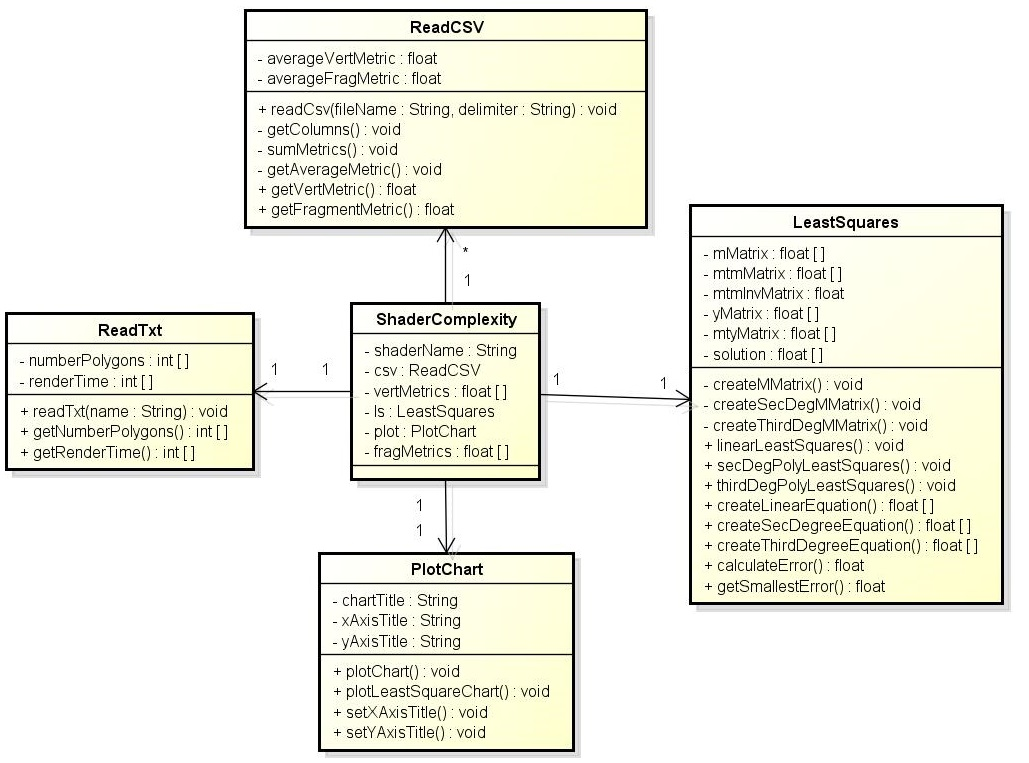
\includegraphics[keepaspectratio=true,scale=0.58]{figuras/minquad_diag.jpg}
	\caption{Diagrama de Classes do \textit{script} de automatização}
	\label{minquad_diag}
	\end{figure}

